\chapter{Data Source}
\label{chap:XXXX}

In this chapter we answer the following question: \emph{What are the security gains from using diverse \glspl{os} on a replicated intrusion-tolerant system?}
To answer this question we have analyzed to what extent different \glspl{os} share common vulnerabilities.
 

\section{Methodology}

This section presents the methodology adopted in our study, with particular focus on how the data set (i.e., the vulnerabilities) was selected, processed and analyzed.

\emph{Data source. }
We have analyzed OS vulnerability data from the NVD database~\cite{nvd}. NVD uses the CVE definition of vulnerability \cite{cveterminology}, which is given below:
%\vspace*{-4ex}
\begin{quote}
  \begin{definition}[CVE Vulnerability]
    An information security ``vulnerability'' is a mistake in software that can be directly used by a hacker to gain access to a system or network.

    CVE considers a mistake a vulnerability if it allows an attacker to use it to violate a reasonable security policy for that system (this excludes entirely ``open'' security policies in which all users are trusted, or where there is no consideration of risk to the system).

    For CVE, a vulnerability is a state in a computing system (or set of systems) that either:
    \begin{itemize}
    \item allows an attacker to execute commands as another user;
    \item allows an attacker to access data that is contrary to the specified access restrictions for that data;
    \item allows an attacker to pose as another entity;
    \item allows an attacker to conduct a denial of service.
    \end{itemize}
  \end{definition}
\end{quote}


NVD aggregates vulnerability reports from more than 70 security companies, forums, advisory groups and organizations\footnote{See the complete list on \url{http://cve.mitre.org/compatible/alerts_announcements.html}.}, being thus the most complete vulnerability database on the web.
All data is made available as XML files containing the reported vulnerabilities on a given period, called \emph{data feeds}.
We analyze feeds from 2002 to 2011\footnote{The 2002 feed includes information about vulnerabilities that were reported between 1994 and 2002. The most recent feed that was analyzed in this paper contained vulnerabilities until the end of  2011.}.



Each NVD data feed contains a list of reported vulnerabilities sorted by its date of publication on a given period.
For each vulnerability, called \emph{entry} in the NVD parlance, interesting information is provided such as: a unique name for the entry, in the format CVE-\textit{YEAR}-\textit{NUMBER}; the list of products (with version numbers) affected by the vulnerability; the date of vulnerability publication; and the security attributes that are affected when the vulnerability is exploited on a system.

We developed a program that collects, parses and inserts the XML data feeds into an SQL database, deployed with a custom schema to group vulnerabilities by affected products and versions.

\emph{Data selection. }
Despite the large amount of information about each vulnerability available in NVD, for the purposes of this study we are only interested in the name, publication date, summary  (description), type of exploit (local or remote), and list of affected configurations.
We have collected vulnerabilities reported for 64 Common Platform Enumerations (CPEs)~\cite{cpe}.
Each one of these describes a system, i.e., a stack of software/hardware components in which the vulnerability may be exploited.
These CPEs were filtered, resulting in the following information that was stored in our database:

\begin{itemize}

\item \textbf{Part:} NVD separates this in Hardware, Operating System and Application. For the purpose of this study we choose only enumerations marked as Operating System;

\item \textbf{Product:} The product name of the platform;

\item \textbf{Vendor:} Name of the supplier or vendor of the product platform.

\end{itemize}


Those 64 CPEs were, by manual analysis, clustered in 11 server-based OS distributions: \textit{OpenBSD, NetBSD, FreeBSD, OpenSolaris, Solaris, Debian, Ubuntu, Red Hat\footnote{\textit{Red Hat} comprises the ``old'' Red Hat Linux (discontinued in 2003) and the newer Red Hat Enterprise Linux (RHEL).}, Windows2000, Windows2003} and \textit{Windows2008}.
These distributions cover the most used \emph{server OS products} of the BSD, Solaris, Linux and Windows families (Mac~OS~X was not included due to its low popularity on the server market -- see, e.g., \cite{w3techs}).

%We did not include Mac~OS~X because, unlike for the included OSes, we did not have an OS~X system available for cross-validation of vulnerability reports.

\begin{figure}[!ht]
 \centering
 \includegraphics[width=0.9\columnwidth]{images/ea-crop.pdf}
 \caption{Simplified SQL schema of the database used to store and analyze the NVD data. Fields not displayed are only used for auxiliary purposes.}
 \label{ea}
\end{figure}

The schema of the resulting database is displayed in Figure \ref{ea}.
%The tables with prefix \textit{cvss}, \textit{vulnerability\_type} and \textit{security\_protection} are employed to optimize the database.
The most important tables are:

\begin{itemize}
\item \emph{cvss\_*} tables: refer directly to the Common Vulnerability Scoring System (CVSS) metrics \cite{cvss} of the stored vulnerabilities, which quantify the severity and impact of vulnerabilities;
\item \emph{vulnerability}: stores basic data about a vulnerability (name, publication date, etc.) from the NVD augmented with vulnerability life cycle information from the Open Source Vulnerability Database (OSVDB) \cite{osvdb};
\item \emph{vulnerability\_type}: stores the vulnerability type assigned by us (see Section \ref{vulntypes});
\item \emph{os}: stores the operating systems platforms of interest in this study;
\item \emph{os\_vuln}: stores the relationship between vulnerabilities and operating systems, and their affected versions.
\end{itemize}

The use of an SQL database brings at least three benefits when compared with analyzing the data directly from the XML feeds.
First, it allows us to \emph{enrich the data set} by hand, for example, by assigning, to each vulnerability, information regarding its type (see Section \ref{vulntypes}), and also by associating release times and family names to each affected OS distribution.
Second, it allows us to modify the CVE fields to correct problems.
For instance, one of the problems with NVD is that the same product is occasionally registered with distinct names in different entries; e.g.,
(\textit{debian\_linux}, \textit{debian}) and (\textit{linux}, \textit{debian}) are two (product, vendor) pairs we have found for the Debian Linux distribution.
This same problem was previously observed by other users of NVD data feeds \cite{cvedetails}.
Finally, an SQL database is much more convenient to work with than parsing the feeds on demand.

\subsection{Filtering the Data}\label{filtering_data}


From the more than 44,000 vulnerabilities published by NVD at the time of this study, we selected 2563 vulnerabilities.
These vulnerabilities are the ones classified as OS-level vulnerabilities (``/o'' in their CPE) for the operating systems under consideration.

When manually inspecting the data set, we discovered and removed vulnerabilities that contained tags in their descriptions such as \emph{Unknown} and \emph{Unspecified}. These correspond to vulnerabilities for which NVD does not know exactly where they occur or why they exist (however, they are usually included in the NVD database because they were mentioned in some patch released by a vendor). We also found few vulnerabilities flagged as \emph{**DISPUTED**}, meaning that product vendors disagree with the vulnerability existence, and \emph{Duplicate}, used for vulnerabilities in which the \emph{summary} points to a duplicate entry or duplicate entry suspicion.
Due to the uncertainty that surrounds these vulnerabilities, we decided to exclude them from the study as well.

Table \ref{tab:unknowns} shows the distribution of these vulnerabilities across the analyzed OSes, together with the total number of valid vulnerabilities.

%TABLE 1
\begin{table}[!ht]
\caption{Distribution of OS vulnerabilities in NVD.}
\label{tab:unknowns}
\begin{center}
{\scriptsize
\begin{tabular}{|l||c | c | c | c | c|}\hline
\textbf{OS} & \textbf{Valid} & \textbf{Unknown} & \textbf{Unspecified} & \textbf{Disputed} & \textbf{Duplicate}  \\\hline\hline % total
OpenBSD & 153 & 1 & 1 & 1 & 0 \\
NetBSD & 143 & 0 & 1 & 2 & 0  \\
FreeBSD & 279 & 0 & 0 & 2 & 0 \\
OpenSolaris & 31 & 0 & 52 & 0 & 0  \\
Solaris & 426 & 40 & 145 & 0 & 3  \\
Debian & 213 & 3 & 1 & 0 & 0  \\
Ubuntu & 90 & 2 & 1 & 0 & 0  \\
Red Hat & 444 & 13 & 8 & 1 & 1  \\
Windows2000 & 495 & 7 & 28 & 5 & 5  \\
Windows2003 & 56 & 5 & 34 & 3 & 5  \\
Windows2008 & 334 & 0 & 8 & 0 & 3   \\\hline\hline
\textbf{\#distinct vulns.} & 2270 & 63 & 210 & 8 & 12 \\ \hline
\end{tabular}
}
\end{center}
\end{table}

An important observation about Table \ref{tab:unknowns} is that the columns do not add up to the number of distinct vulnerabilities (last row of the table) because some vulnerabilities are shared among OSes and are counted only once.
Notice that about 60\% of the removed vulnerabilities affected Solaris and OpenSolaris.
Moreover, these two systems are the only ones that have more than 10\% of its vulnerabilities removed.
We should remark that this manual filtering was necessary to increase the confidence that only valid vulnerabilities were used in the study.


\section{OS Diversity Study}\label{study}

This section describes the results of the study. It provides an overall analysis of the counts of vulnerabilities in each OS component class, presents vulnerabilities that are common to OS pairs, and shows the evolution of shared OS vulnerabilities over time. The section also gives empirical evidence to demonstrate that there are security gains in using diverse OSes in a replicated system.


\subsection{Vulnerability Distribution by OS Component}\label{vulntypes}

Nowadays, when users acquire or download an operating system, they get a kernel implementing the fundamental OS functionality but also a number of other software components.  After the initial installation, users may reconfigure the machine to their needs, for instance by removing application packages that are unnecessary and/or by including device drivers to support new hardware. This customization is also advisable from a security standpoint, with a few different baseline OS installations created for machines with distinct roles within an organization. For example, a network server OS installation should be stripped of most applications to minimize the attack surface and reduce the risk of intrusion. Therefore, besides understanding how vulnerabilities affect the various operating system products, it is also important to know what parts of these systems are compromised by the vulnerabilities. In NVD, an \emph{operating system product} is composed by the kernel, device drivers, optional modules, system software and applications. Since NVD does not have a specific field identifying the affected component except for the vulnerability description, we inspected the entries manually and classified each vulnerability in one of four categories: \textit{Driver, Kernel, System Software} and \textit{Application}. %The rationale for this classification is the %following:
The classification criteria are the following:

\begin{itemize}

\item \textbf{Kernel:} vulnerabilities in the TCP/IP stack (and other network protocols implemented in the OS), file system, process and task management, core libraries and modules related to the CPU architecture;

\item \textbf{Driver:} vulnerabilities in drivers for the devices that might be connected to the machine (for example, wireless/wired network cards, video/graphic cards, web cams, audio cards, plug and play devices);

\item \textbf{System Software:} vulnerabilities in software providing common OS functionalities such as login, shells and basic daemons (e.g., DNS, telnet, lpd). In this class, we only account for software that comes by default with the distribution (although sometimes it is possible to uninstall these components without affecting the main OS operation);

\item \textbf{Application:} vulnerabilities in software that comes with the OS but that is not needed for basic operation, and in some cases requires specific installation. For example, database management systems, messaging clients, text editors and processors, web/email/FTP clients and servers, music/video players, programming languages (compilers and virtual machines), security packages (antivirus and authentication solutions), and games.
\end{itemize}


Table~\ref{tab:classification} summarizes the result of the analysis of the 2270 vulnerability descriptions, which were then assigned to one of the OS component classes. The table shows that, with the exception of \textit{Drivers}, all OS products have a reasonable number of vulnerabilities in each class.  Therefore, this confirms the intuition that there are security gains if certain software components can be removed from the OS distributions. In the BSD and Solaris families, vulnerabilities appear in high numbers in the \textit{Kernel} part, while in the Linux and Windows families, the \textit{Applications} vulnerabilities are more prevalent. This can be explained by noticing that Windows and Linux default distributions usually contain more pre-installed applications when compared to BSD/Solaris. Therefore, the number of \textit{Applications} vulnerabilities in Windows and Linux have higher reported values -- there is the expectation that users will not install most of the applications missing from  the default distributions, and thus their vulnerabilities not appear in the OS statistics.



%TABLE 2
\begin{table}[!ht]
\caption{Vulnerabilities per OS component class.}
\label{tab:classification}
\begin{center}
{\scriptsize
\begin{tabular}{|l||c|c|c|c||c|}\hline
\textbf{OS} & \textbf{Driver} & \textbf{Kernel} & \textbf{Sys. Soft.} & \textbf{Application} & \textbf{Total}  \\ \hline\hline
OpenBSD 			& 2	 	& 76 		& 37 	& 38 	& 153 \\ %\hline
NetBSD			 	& 9 	& 64 		& 39 	& 31 	& 143 \\ %\hline
FreeBSD 			& 4 	& 153 	& 61	& 61 	& 279 \\ %\hline
OpenSolaris 	& 0 	& 15 		& 9 	& 7 	& 31\\ %\hline
Solaris 			& 2		& 155		& 120	& 149 & 426\\ %\hline
Debian 			& 1 	& 25 		& 39 	& 148 & 213 \\ %\hline
Ubuntu 			& 2 	& 22 		& 8 	& 58 	& 90 	\\ %\hline
Red Hat 			& 5 	& 94  	& 108 & 237 & 444 \\ %\hline
Windows2000     & 3 	& 146	 	& 135 & 211 & 495 \\
Windows2003     & 2 	& 171 	& 96 & 291 & 560 \\
Windows2008     & 0 	& 123 	& 36	& 175	& 334 \\  \hline\hline
\textbf{\% Total} 	& 1.0\% & 33.5\% & 22.5\% & 42.9\% &  \\  \hline
% driver 23 kernel 761 prim soft 511 app 975
%total 2270
\end{tabular}
}
\end{center}
\end{table}

The last row of the table presents the percentage of each class on the total data set. One can observe that most vulnerabilities occur in the Application and Kernel components, which is then followed by the System Software group of utility programs. It is interesting to notice that Drivers have a very small percentage of the published OS vulnerabilities. This result is somewhat surprising because device drivers account for a large fraction of OS code~\cite{Chou01}, and since they are typically hard to develop, one would expect that they would contain a large number of programming flaws. In fact, previous studies have demonstrated that drivers are the major cause for crashes in certain OSes~\cite{Gan06}. One, however, should keep in mind that software bugs do not necessarily translate into security vulnerabilities, which are the kind of flaw reported in the NVD\@. In order to become vulnerabilities, the adversary has to be able to force the conditions to activate the bugs, which for device drivers can be extremely difficult because they are related to specific low-level aspects of the system.


\subsection{Common Vulnerabilities}\label{common_vulns}

This section analyzes the vulnerabilities that were shared in OS pairs over the period of 1994 to 2011. In the investigation, we consider three possible server machine setups offering an increasingly more secure platform. This accommodates the case where system administrators create differentiated OS installations, which contain more or less vulnerabilities depending on the services and applications available in the server. Of course, other setups could be used, but we decided to concentrate on these configurations because they are quite generic and they lead to results that can be directly obtained from the NVD data. The setups are the following:

\begin{itemize}

\item \textbf{Fat Server:} The server contains most of the software packages for a given OS, and consequently, it can be used to run various kinds of applications by locally or remotely connected users. This server has potentially all vulnerabilities that were reported for the corresponding OS;

\item \textbf{Thin Server:} This setting corresponds to a platform that does not contain any applications (with the exception of the replicated service). The server has a decreased security risk because the attack vectors related to applications have been mostly eliminated. In this setting, vulnerabilities classified as \textit{Applications} are excluded from the statistics (see Section~\ref{vulntypes});

\item \textbf{Isolated Thin Server:} The server is configured similarly to the Thin Server but is placed in a room physically protected from illegal accesses, with remote logins disabled, and therefore it can only be compromised by receiving malicious packets from the network. In this setting, we only consider remotely exploitable vulnerabilities (those with ``Network'' or ``Adjacent Network'' values in their CVSS\_ACCESS\_VECTOR field) that are not classified as \textit{Applications}.

\end{itemize}

The Fat Server setup corresponds to a case where any application available in the OS distribution may be targeted by attack. Therefore, it provides an upper bound estimate on the number of vulnerabilities that can be exploited. The Thin Server setups (Isolated or not) are the counterpart case, where the system is deployed without applications that come bundled with the OS, and thus provide a lower bound estimate on the number of common vulnerabilities. The Isolated Thin Server, in particular, only has the vulnerabilities that can be remotely exploited. Of course, in practice, at least one application (such as a name service or a distributed file service) would be deployed in an intrusion-tolerant system, and the vulnerabilities of this application would add up to the flaws that we will report. In any case, since we expect that most of the complexity is in the operating system, we anticipate that a single application will have a small contribution to the overall number of vulnerabilities.

% The setup with a Fat Server corresponds to a case where all % applications available in the OS distribution can be attacked by the % adversary. Therefore, it provides an estimation of a high bound on the % number of vulnerabilities that can be exploited. The setups with Thin % Servers (Isolated or not) are the counterpart case where the system is % configured without applications, and therefore they provide an % estimate of a lower bound on the number of common vulnerabilities. The % Isolated Thin Server, in particular, only has the vulnerabilities that % can be remotely exploited. Of course, in practice, at least one % application (such as, a name or a distributed file service) would be % deployed in the intrusion tolerant system, and the vulnerabilities of % this application would add up to the flaws that we will report. In any % case, since we expect that most of the complexity is in the operating % system, we anticipate that the single application will have a small % contribution to the overall number of vulnerabilities.

Table~\ref{tab:vulns} shows the vulnerabilities that were found in common for every combination of OS pair.
In all cases, the number of shared vulnerabilities between two OSes is substantially reduced when compared to the overall set of vulnerabilities. Even considering a Fat Server configuration, it is possible to find out OS pairs that do not have common flaws (e.g., NetBSD-Ubuntu), and OS families that share very few vulnerabilities (e.g., BSD and Windows). As expected, OSes from the same family have more common vulnerabilities due to the software components and applications that are reused (e.g., Debian-Red Hat or Windows2000-Windows2003). The Thin Server when compared with the Fat Server shows improvements in several OS pairs, but often there are still a few shared flaws. In contrast, the use of an Isolated Thin Server has a much stronger impact on security because it substantially diminishes the number of common vulnerabilities -- the number of pairs with zero vulnerabilities goes from 11 to 21. Overall, this means that a significant portion of common vulnerabilities are local (i.e., cannot be exploited remotely) and/or come from applications that are available in both operating systems.

%TABLE III
\begin{table*}[!ht]
\caption{Vulnerabilities (1994 to 2011): \emph{Fat Server} - all vulnerabilities; \emph{Thin Server} - no application vulnerabilities; \emph{Isolated Thin Server} - no application vulnerabilities and only remotely-exploitable vulnerabilities. The columns with \textit{v(A)} and \textit{v(B)} show the total number of vulnerabilities collected for OSes A and B respectively, whereas \textit{v(A,B)} is the count of vulnerabilities that affect both the A and B systems.}
\label{tab:vulns}
\begin{center}
{\scriptsize
\begin{tabular}{|l|| c c c| c c c| c c c| }%\hline

 \multicolumn{1}{c}{\textbf{Operating Systems}} &
 \multicolumn{3}{c}{\textbf{Fat Server}} &
 \multicolumn{3}{c}{\textbf{Thin Server}} &
 \multicolumn{3}{c}{\textbf{Isolated Thin Server}} \\
\hline
Pairs (A-B) & $\mathit{v}(A)$ & $\mathit{v}(B)$ & $\mathit{v}(A,B)$ & $\mathit{v}(A)$ & $\mathit{v}(B)$ & $\mathit{v}(A,B)$& $\mathit{v}(A)$ & $\mathit{v}(B)$ & $\mathit{v}(A,B)$\\\hline\hline
OpenBSD-NetBSD & 153 & 143 & 45 & 115 & 112 & 34 & 62 & 46 & 17\\
OpenBSD-FreeBSD & & 279 & 57 & & 218 & 49 & & 90 & 33\\
OpenBSD-OpenSolaris & & 31 & 1 & & 24 & 1 & & 6 & 0\\
OpenBSD-Solaris & & 426 & 13 & & 277 & 10 & & 108 & 6\\
OpenBSD-Debian & & 213 & 2 & & 65 & 2 & & 28 & 0\\
OpenBSD-Ubuntu & & 90 & 3 & & 32 & 1 & & 10 & 0\\
OpenBSD-Red Hat & & 444 & 11 & & 207 & 6 & & 69 & 4\\
OpenBSD-Win2000 & & 495 & 3 & & 284 & 3 & & 183 & 3\\
OpenBSD-Win2003 & & 560 & 2 & & 269 & 2 & & 138 & 2\\
OpenBSD-Win2008 & & 334 & 1 & & 159 & 1 & & 56 & 1\\ \hline
NetBSD-FreeBSD & 143 & 279 & 54 & 112 & 218 & 41 & 46 & 90 & 25\\
NetBSD-OpenSolaris & & 31 & 0 & & 24 & 0 & & 6 & 0\\
NetBSD-Solaris & & 426 & 18 & & 277 & 14 & & 108 & 10\\
NetBSD-Debian & & 213 & 5 & & 65 & 4 & & 28 & 4\\
NetBSD-Ubuntu & & 90 & 0 & & 32 & 0 & & 10 & 0\\
NetBSD-Red Hat & & 444 & 12 & & 207 & 9 & & 69 & 6\\
NetBSD-Win2000 & & 495 & 3 & & 284 & 3 & & 183 & 3\\
NetBSD-Win2003 & & 560 & 1 & & 269 & 1 & & 138 & 1\\
NetBSD-Win2008 & & 334 & 1 & & 159 & 1 & & 56 & 1\\ \hline
FreeBSD-OpenSolaris & 279 & 31 & 0 & 218 & 24 & 0 & 90 & 6 & 0\\
FreeBSD-Solaris & & 426 & 23 & & 277 & 15 & & 108 & 8\\
FreeBSD-Debian & & 213 & 7 & & 65 & 4 & & 28 & 1\\
FreeBSD-Ubuntu & & 90 & 3 & & 32 & 3 & & 10 & 0\\
FreeBSD-Red Hat & & 444 & 20 & & 207 & 13 & & 69 & 5\\
FreeBSD-Win2000 & & 495 & 4 & & 284 & 4 & & 183 & 4\\
FreeBSD-Win2003 & & 560 & 2 & & 269 & 2 & & 138 & 2\\
FreeBSD-Win2008 & & 334 & 1 & & 159 & 1 & & 56 & 1\\ \hline
OpenSolaris-Solaris & 31 & 426 & 27 & 24 & 277 & 22 & 6 & 108 & 6\\
OpenSolaris-Debian & & 213 & 1 & & 65 & 1 & & 28 & 0\\
OpenSolaris-Ubuntu & & 90 & 1 & & 32 & 1 & & 10 & 0\\
OpenSolaris-Red Hat & & 444 & 1 & & 207 & 1 & & 69 & 0\\
OpenSolaris-Win2000 & & 495 & 0 & & 284 & 0 & & 183 & 0\\
OpenSolaris-Win2003 & & 560 & 0 & & 269 & 0 & & 138 & 0\\
OpenSolaris-Win2008 & & 334 & 0 & & 159 & 0 & & 56 & 0\\   \hline
Solaris-Debian & 426 & 213 & 4 & 277 & 65 & 4 & 108 & 28 & 2\\
Solaris-Ubuntu & & 90 & 2 & & 32 & 2 & & 10 & 0\\
Solaris-Red Hat & & 444 & 17 & & 207 & 10 & & 69 & 6\\
Solaris-Win2000 & & 495 & 10 & & 284 & 3 & & 183 & 3\\
Solaris-Win2003 & & 560 & 8 & & 269 & 1 & & 138 & 1\\
Solaris-Win2008 & & 334 & 1 & & 159 & 0 & & 56 & 0\\  \hline
Debian-Ubuntu & 213 & 90 & 15 & 65 & 32 & 6 & 28 & 10 & 2\\
Debian-Red Hat & & 444 & 66 & & 207 & 28 & & 69 & 13\\
Debian-Win2000 & & 495 & 1 & & 284 & 1 & & 183 & 1\\
Debian-Win2003 & & 560 & 1 & & 269 & 1 & & 138 & 1\\
Debian-Win2008 & & 334 & 0 & & 159 & 0 & & 56 & 0\\ \hline
Ubuntu-Red Hat & 90 & 444 & 28 & 32 & 207 & 8 & 10 & 69 & 1\\
Ubuntu-Win2000 & & 495 & 1 & & 284 & 1 & & 183 & 1\\
Ubuntu-Win2003 & & 560 & 1 & & 269 & 1 & & 138 & 1\\
Ubuntu-Win2008 & & 334 & 0 & & 159 & 0 & & 56 & 0\\ \hline
Red Hat-Win2000 & 444 & 495 & 2 & 207 & 284 & 1 & 69 & 183 & 1\\
Red Hat-Win2003 & & 560 & 2 & & 269 & 1 & & 138 & 1\\
Red Hat-Win2008 & & 334 & 0 & & 159 & 0 & & 56 & 0\\  \hline
Win2000-Win2003 & 495 & 560 & 265 & 284 & 269 & 120 & 183 & 138 & 85\\
Win2000-Win2008 & & 334 & 80 & & 159 & 29 & & 56 & 16\\  \hline
Win2003-Win2008 & 560 & 334 & 282 & 269 & 159 & 125 & 138 & 56 & 40\\ \hline
\end{tabular}
}
\end{center}
\end{table*}



Table~\ref{tab:class-pairs} shows which parts of the OS are affected by common vulnerabilities in an Isolated Thin Server configuration, considering only the OS pairs with non-zero common vulnerabilities. The fact that there are many shared \textit{Kernel} and \textit{System Software} vulnerabilities between Windows2000 and Windows2003 indicates that the latter inherits considerable parts of the OS from its predecessor. This same trend is also observed between Windows2008 and Windows2003/Windows2000, although to a less extent. Interestingly, no single vulnerable driver is present in all products, which can be explained by the very few faulty drivers that are reported.

%Table 4
\begin{table}[!ht]
\caption{Common vulnerabilities on Isolated Thin Servers (only OS pairs with non-zero shared flaws).}
\label{tab:class-pairs}
\begin{center}
{\scriptsize
\begin{tabular}{|l||c|c|c||c|}\hline
OS Pairs & \emph{Driver} & \emph{Kernel} & \emph{Sys. Soft.} & \emph{Total}\\\hline\hline
Win2000-Win2003 &  0 & 42 & 43 & 85 \\\hline
Win2003-Win2008 &  0 & 18 & 22 & 40  \\\hline
OpenBSD-FreeBSD &  1 & 14  &  18 & 33  \\\hline
NetBSD-FreeBSD &  2 & 13 & 10 & 25  \\\hline
OpenBSD-NetBSD  & 1 & 8 & 8 & 17\\\hline
Win2000-Win2008 &  0 & 8 & 8 & 16  \\\hline
Debian-Red Hat &  0 & 5 & 8 & 13  \\\hline
NetBSD-Solaris &  0 & 4 & 6 & 10  \\\hline
FreeBSD-Solaris &  0 & 5 & 3 & 8  \\\hline
OpenSolaris-Solaris &  0 & 3 & 3 & 6  \\\hline
OpenBSD-Solaris  &  0 & 5 & 1 & 6  \\\hline
Solaris-Red Hat &  0 & 3 & 3 & 6  \\\hline
NetBSD-Red Hat &  0 & 0 & 6 & 6  \\\hline
FreeBSD-Red Hat &  0 & 1 & 4 & 5 \\\hline
OpenBSD-Red Hat &  0 & 1 &  3 & 4  \\\hline
NetBSD-Debian &  0 & 0 & 4 & 4  \\\hline
FreeBSD-Win2000 &  1 & 3 & 0 & 4  \\\hline
OpenBSD-Win2000 &  0 & 3 &  0 & 3  \\\hline
NetBSD-Win2000 &  1 & 2 & 0 & 3  \\\hline
Solaris-Win2000 &  0 & 3 & 0 & 3  \\\hline
OpenBSD-Win2003 &  0 & 2 & 0 & 2  \\\hline
FreeBSD-Win2003 &  0 & 2 & 0 & 2  \\\hline
Solaris-Debian &  0 & 1 & 1 & 2  \\\hline
Debian-Ubuntu &  0 & 0 & 2 & 2  \\\hline
NetBSD-Win2003 &  0 & 1 & 0 & 1  \\\hline
NetBSD-Win2008 &  0 & 1 & 0 & 1  \\\hline
FreeBSD-Debian &  0 & 0 & 1 & 1 \\\hline
FreeBSD-Win2008 &  0 & 1 & 0 & 1  \\\hline
Debian-Win2000 &  0 & 0 & 1 & 1  \\\hline
Ubuntu-Red Hat &  0 & 0 & 1 & 1  \\\hline
Ubuntu-Win2000 &  0 & 0 & 1 & 1  \\\hline
Red Hat-Win2000 &  0 & 0 & 1 & 1  \\\hline
OpenBSD-Win2008 &  0 & 1 & 0 & 1  \\\hline
Solaris-Win2003 &  0 & 1 & 0 & 1  \\\hline
Debian-Win2003 &  0 & 0 & 1 & 1  \\\hline
Ubuntu-Win2003 &  0 & 0 & 1 & 1  \\\hline
Red Hat-Win2003 &  0 & 0 & 1 & 1  \\\hline
\end{tabular}
}
\end{center}
\end{table}

The second OS family with more common vulnerabilities is BSD, which also reuses several OS components. Here, a few vulnerabilities were found in device drivers that appear in more than one OS pair. A somewhat surprising result is the fact that most Linux distributions have much less shared flaws than we anticipated. We inspected the vulnerabilities manually in order to find an explanation, and we discovered that Linux distributions customize both their kernel and system software, and thus the vulnerabilities are less common. Another interesting point about OSes from the Linux family is that they have an almost negligible number of driver vulnerabilities (see Table \ref{tab:classification}), and none of them appears in more than one OS.


OpenSolaris is an open source operating system based on Solaris that was released in 2008, and until this moment the two OSes only share a small number of vulnerabilities.


Intrusion-tolerant systems are usually built using four or more replicated servers. Therefore, it is useful to understand if there are many vulnerabilities that involve groups of OSes larger than two -- if this is the case, then it will be hard to find OS configurations for the various servers that do not share vulnerabilities, and a goal of using off-the-shelf diversity will be difficult to be achieved in practice. Figure \ref{top} portrays the number of common vulnerabilities that exist simultaneously in increasingly larger sets of operating systems (with Isolated Thin Servers). The graph shows a rapid decrease of the shared vulnerabilities as the number of OSes grows. The largest group that was affected by the same vulnerability had six OSes, and this occurred only for a single flaw, and there were also two vulnerabitlities in sets with five OSes. Vulnerabilities in two and three OSes normally occur in systems from the same family, whose common ancestry implies the reuse of larger portions of the code base. As we have seen in previous tables, this is particularly true for the Windows and BSD families.

\begin{figure}[!ht]
 \centering
 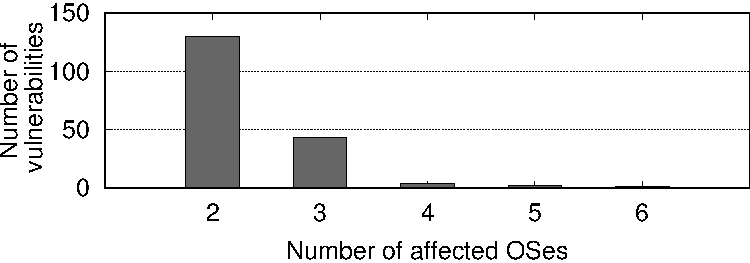
\includegraphics[scale=0.5]{images/top.pdf}
 \caption{Common vulnerabilities for $n$ different OSes (with Isolated Thin Servers).}
 \label{top}
\end{figure}


Table \ref{tab:spreaded_vulns} lists in more detail the vulnerabilities that can be exploited in larger groups (four to six) of OSes. The first three bugs have a considerable impact because they allow a remote adversary to run arbitrary commands on the local system using a high-privilege account. They occurred either in widespread login services (telnet and rlogin) or in a basic system function, and consequently several products from the BSD family were affected, as well as Solaris. The NVD entry for the CVE-2001-0554 vulnerability also had external references to the Debian and Red Hat websites, which could indicate that these systems might suffer from a similar (or the same) problem. Vulnerability CVE-2008-1447 occurs in a large number of systems because it results from a bug in the BIND implementation of the Domain Name System (DNS). Since BIND is a highly popular service, more OSes could potentially be affected. A closer look at the corresponding NVD entry reveals external references to the sites of OpenBSD, NetBSD, and FreeBSD, indicating that they would be vulnerable in case this software was being used. This sort of vulnerability confirms that from an intrusion-tolerance perspective it is unwise to run the same server software everywhere, and that diverse implementations must be selected (in this case for recursive DNS servers).

\begin{table}[!ht]
\caption{Vulnerabilities that affect more than four OSes.}
\label{tab:spreaded_vulns}
\begin{center}
{\scriptsize
\begin{tabular}{|c||c| p{7,8cm} | }\hline
\textbf{CVE} & \#affected OSes  & Description  \\\hline\hline
CVE-1999-0046  &  4  & Buffer Overflow of \emph{rlogin} allows admin access. Affects: NetBSD, FreeBSD, Solaris and Debian. \\ \hline
CVE-2001-0554  &  4  & Buffer overflow in telnetd (telnet daemon) allows remote attackers to execute arbitrary commands. Affects: OpenBSD, NetBSD, FreeBSD and Solaris.  \\ \hline
CVE-2003-0466  &  4  & Off-by-one error in the Kernel function \emph{fb\_realpath()} allows admin access. Affects: OpenBSD, NetBSD, FreeBSD and Solaris.  \\ \hline
CVE-2005-0356  &  4  & TCP implementations allow a denial of service (DoS) via spoofed packets with large timer values, when used with Protection Against Wrapped Sequence Numbers. Affects: OpenBSD, FreeBSD, Windows2000 and Windows2003. \\ \hline
CVE-2008-1447  &  5  & The BIND 8 and 9 implementation of the DNS protocol allow attackers to spoof DNS traffic via a birthday attack to conduct cache poisoning against recursive resolvers. Affects: Debian, Ubuntu, Red Hat, Windows2000 and Windows2003.  \\ \hline
CVE-2001-1244  &  5  & TCP implementations allow a DoS by setting a maximum segment size very small to force the generation of more packets, amplifying network traffic and CPU consumption. Affects: OpenBSD, NetBSD, FreeBSD, Solaris and Windows2000. \\ \hline
CVE-2008-4609  &  6  & TCP implementation allows a DoS via multiple vectors that manipulate TCP state table. Affects: OpenBSD, NetBSD, FreeBSD, Windows2000, Windows2003 and Windows2008.   \\ \hline
\end{tabular}
}
\end{center}
\end{table}


The remaining three vulnerabilities are related to the TCP/IP protocol stack. All of them affect system availability, allowing different forms of denial of service (DoS) attacks. CVE-2008-4609 is the vulnerability that affects more operating systems, according to the NVD database. Given that TCP/IP stack code is often reused across operating systems, we checked the web sites of the other OSes for reports related to this vulnerability. We only found a disclaimer by Red Hat~\cite{RH-CVE-2008-4609} stating that this flaw affected some releases but that they would not provide an update (they only offered a mitigation solution based on IPtables, the Linux firewall software).

Overall, the above results look encouraging because over a large period of time (around 18 years) there are very few vulnerabilities that appear in many operating systems. A good portion of them are in the TCP/IP stack implementation, which is probably the most shared software component across OSes, but they only impact on the availability of the system, leaving confidentiality and integrity of data unharmed.



\section{Strategies for OS Diversity Selection}\label{evaluation}

This section presents three alternative strategies to deploy diverse operating systems on replicated systems, to decrease the chance of common vulnerabilities. We start the section by first describing an approach we called the Common Vulnerability Indicator (CVI), which is used by one of the strategies. For each strategy, we then give example sets of OSes that exhibit a good level of diversity, and perform an evaluation based on the collected data. Finally we conclude the section with an analysis of potential diversity between releases of the same OSes (concentrating on the OSes that the three strategies picked as the best configuration).

\subsection*{Common Vulnerability Indicator}\label{cvi}

We already saw in the previous section that the number of common vulnerabilities that are observed between different operating systems varies over time. In order to be able to evaluate which OS pairs are more (or less) likely to experience common flaws while taking into account the timing of vulnerability disclosures, we developed a new metric, called the \emph{Common Vulnerability Indicator (CVI)}. This indicator is calculated for a given year $y$, based on the vulnerabilities that were shared by operating systems A and B over a period of $\mathit{tspan}$ previous years. CVI is built to ensure the following desirable properties:
\begin{enumerate}
\newcommand{\OLDtheenumi}{\theenumi}
\renewcommand{\theenumi}{\roman{enumi}}
\item $\mathit{CVI}_y(A,B) = 0$ if A and B have no common vulnerabilities in the $\mathit{tspan}$ interval;
\item $\mathit{CVI}_y(A,B) < \mathit{CVI}_y(C,D)$ if A and B shared less vulnerabilities than C and D in each year of the considered period;
\item $\mathit{CVI}_y(A,B) < \mathit{CVI}_y(C,D)$ if A and B had $N$ common vulnerabilities in the distant past while C and D had $N$ shared vulnerabilities more recently;
\item $\mathit{CVI}_{y_2}(A,B) < \mathit{CVI}_{y_1}(A,B)$, with $y_1 < y_2$, if the number of common vulnerabilities for A and B has decreased over the years.
\renewcommand{\theenumi}{\OLDtheenumi}
\end{enumerate}
Therefore, CVI is useful for comparison purposes, allowing the identification of OS pairs that have a smaller number of common flaws, while taking into consideration the instant when vulnerabilities were found. This last point is particularly important because operating systems are constantly evolving, potentially getting more (or less) diverse, and consequently, one should take into consideration the time dimension when selecting OS configurations (e.g., OS pairs that have had less common flaws recently are likely better candidates).

CVI is computed as follows:

\begin{itemize}

\item First, a weighting factor $\alpha_{i}$ is defined for each year   $i \in \{y-\mathit{tspan}+1, ..., y-2, y-1, y\}$,

\begin{equation}
\alpha_{i} = 1 - \frac{y-i}{\mathit{tspan}}
\end{equation}

\item CVI is then obtained using the number of vulnerabilities $v_{i}(A,B)$ that appeared in both operating systems A and B for every year $i$ from the start of the time span up to reference year $y$,

\begin{equation}
\mathit{CVI}_{y}(A,B)= \sum_{i = y-\mathit{tspan}+1}^{y} \alpha_{i}\cdot v_{i}(A,B)
\end{equation}

\end{itemize}


Table~\ref{tab:cvi-2011-2009} presents CVI values for the years 2009 to 2011. We have excluded from this analysis OSes with vulnerability information missing for more than one year over the period, to avoid using incomplete data in the calculation of the indicators. Therefore, the following operating systems were not considered in Table~\ref{tab:cvi-2011-2009}: Windows2003, Windows2008, Ubuntu, and OpenSolaris. The CVI values are computed for a $\mathit{tspan}$ of 10 years to reflect a reasonable history. It is possible to see that, with the exception of one system (Solaris with FreeBSD/Red Hat/Windows2000 in the Fat Server), in all remaining cases CVI shows a decreasing trend. Several of the OSes that have evolved over a large period are having less reported vulnerabilities, and this causes a decline in shared vulnerabilities in the recent years. For some of the OS pairs the drop in the CVI value is quite significant, becoming almost one third of the 2009 value (NetBSD with Debian or Red Hat). In the Isolated Thin Server case, there are three pairs with $\mathit{CVI}(A,B)=0$, which shows that they have shared no vulnerabilities during the past 12 years, and are thus particularly good candidates to include in intrusion-tolerant configurations. These systems are Debian with either OpenBSD or FreeBSD or Solaris.

An example of the usefulness of CVI can be seen, e.g., when comparing OpenBSD-Red Hat with Solaris-Red Hat. According to Table~\ref{tab:pairs_vulns_by_year}, both OS pairs had 10 common vulnerabilities in the 2000--2011 period, suggesting that they both provide the same degree of diversity. However, from the CVI values in Table~\ref{tab:cvi-2011-2009}, it is apparent that OpenBSD and Red Hat have become more diverse, in recent years, than Red Hat and Solaris, making it advisable, from a diversity standpoint, to choose the former OS pair over the latter.

\begin{table}[!ht]
\caption{CVI for the years 2009 to 2011, with $\mathit{tspan}$ of 10 years.}
\label{tab:cvi-2011-2009}
\begin{center}
{\scriptsize
\begin{tabular}{|l|c c c|| c c c |}
\cline{2-7}
\multicolumn{1}{c}{} &  \multicolumn{3}{|c||}{\textbf{Fat Server}}  &  \multicolumn{3}{|c|}{\textbf{Isolated Thin Server}} \\ \hline
OS             & 2009 &	2010 & 	2011        & 	2009 & 	2010 & 2011 \\ \hline
OpenBSD-NetBSD  & 17.1 & 13.8 & 14.8        & 8.4 & 7.1 & 6.9   \\
OpenBSD-FreeBSD & 22.2 & 18.0 & 18.1        & 14.1  & 11.6 & 10.3  \\
OpenBSD-Solaris & 4.0 & 3.1 & 3.3           &  1.8 & 1.4 & 0.9  \\
OpenBSD-Debian  & 1.7 & 1.5 & 1.4           &  0.0 & 0.0 & 0.0  \\
OpenBSD-Red Hat & 5.0 & 4.1 & 3.2           &  1.6 & 1.4 & 1.1  \\
OpenBSD-Win2000 & 1.8 & 1.5 & -             &  1.8 & 1.5 & -  \\  \hline
NetBSD-FreeBSD  & 19.7 & 18.3 & 18.8        & 11.0 & 9.3 & 8.6 \\
NetBSD-Solaris  & 4.9 & 4.0 & 4.2           &  1.5 & 1.1 & 0.7  \\
NetBSD-Debian   & 1.4 & 0.9 & 0.5           &  0.6 & 0.4 & 0.2  \\
NetBSD-Red Hat  & 1.8 & 1.1 & 0.5           &  0.6 & 0.4 & 0.2  \\
NetBSD-Win2000  & 1.6 & 1.4 & -             & 1.6 & 1.4 & -   \\ \hline
FreeBSD-Solaris & 6.5 & 5.4 & 6.3           & 2.3 & 1.7 & 1.2  \\
FreeBSD-Debian  & 1.3 & 0.8 & 0.5           & 0.0 & 0.0 & 0.0  \\
FreeBSD-Red Hat & 5.6 & 4.4 & 3.3           & 1.7 & 1.4 & 1.1  \\
FreeBSD-Win2000 & 2.3 & 1.9 & -             & 2.3 & 1.9 & -  \\ \hline
Solaris-Debian  & 1.0 & 0.8 & 0.6           & 0.0 & 0.0 & 0.0  \\
Solaris-Red Hat & 5.3 & 6.5 & 5.5           & 1.0 & 0.7 & 0.5  \\
Solaris-Win2000 & 5.5 & 5.7 & -             & 1.0 & 0.7 & -  \\ \hline
Debian-Red Hat  & 26.1 & 20.5 & 15.7        & 3.2 & 2.1 & 1.4  \\
Debian-Win2000  & 0.9 & 0.8 & -             & 0.9 & 0.8 & -   \\ \hline
Red Hat-Win2000 & 1.8 & 1.6 & -             & 0.9 & 0.8 & -   \\ \hline
\end{tabular}
}
\end{center}
\end{table}



\subsection*{Building Replicated Systems with Diversity}
\label{build_diversity}
This section describes three strategies for choosing diverse sets of operating systems. These strategies utilize the data analyzed earlier as a basis to make decisions, by assuming that the information reported by NVD on vulnerabilities can be correlated to the amount of diversity among OSes. Of course there are some caveats associated with this approach, which we discuss in Section~\ref{limitations}, but the alternatives can be even harder to put in practice, especially if one wants to consider a large number of operating systems. For example, for closed systems (e.g., Windows) it is very difficult to actually determine the level of sharing of OS components, and therefore, diversity estimations based on the code cannot be performed. Moreover, even if this estimate could be obtained, there is the risk that it does not reflect the number of vulnerabilities that occur simultaneously in several operating systems (e.g., two distinct implementations of the same flawed algorithm are vulnerable).

The first strategy, called \emph{Common Vulnerability Count Strategy (CVCst)}, is based on raw data collected over a large interval, and is the simplest approach for selecting OS pairs. It should be used when one wants to treat all vulnerabilities, regardless of the time which were reported, as equally important to make choices. The second strategy, \emph{Common Vulnerability Indicator Strategy (CVIst)}, uses the CVI described in the previous section to select OS pairs taking into account the incidence of common vulnerabilities over the years. It is indicated when one wants to give greater importance to more recent vulnerabilities, because it is a weighted sum. The third strategy, \emph{Inter-reporting Times Strategy (IRTst)}, follows a different approach from the previous ones, focusing not so much on common vulnerabilities directly, but on the frequency in which vulnerabilities appear in the two OSes. If one wants to give more importance to the time interval between successive reports of common vulnerabilities, this is the best strategy. Since this last criterion complements the previous two, one could explore strategies CVCst and CVIst in conjunction with IRTst.

For every strategy, we present example OS sets for the Fat Server and Isolated Thin Server configurations. Fat Server configurations can be pessimistic in the sense that they may account for common vulnerabilities in applications that are not present in the servers, while Isolated Thin Server configurations reflect more accurately the expected setup of dedicated servers in a replicated system. An intrusion-tolerant system usually requires $3f+1$ replicas to tolerate $f$ intrusions (e.g., \cite{Ver03,Cas02,Bessani08:depspace,Mon11}). Therefore, we will focus on sets with four OSes to deploy a hypothetical replicated system with four replicas, which allows one fault to be tolerated.

As a cautious note, one should take into account that Ubuntu and Windows2008 were first released in 2004 and 2008 respectively, so the data for these two OSes was collected for a smaller number of years. Windows2000 is presented in the tables because there are published vulnerabilities until 2010, although it has been gradually  replaced by Windows2003 and Windows2008 in the organizations. Consequently, we do not use Windows2000 when choosing the OS sets. We have excluded OpenSolaris from the study because there is data available for only a limited period. In each strategy and configuration we present two sets: \emph{setCon} is more conservative, since it does not contain Ubuntu and Windows2008; and \emph{setUpdt} is more up-to-date because it can include Ubuntu and Windows2008. When looking at these two sets, one should keep in mind that setCon is selected from a group of OSes for which there is a large amount of NVD data, which contributes for a higher confidence on the result. On the other hand, setUpdt uses OSes with different amounts of NVD data, which can cause small levels of inaccuracy when making comparisons (e.g., in the CVCst, any OS pair featuring Windows2008 has zero common vulnerabilities until 2007). One way to address this would be to only consider vulnerabilities that appear later than 2007 when choosing setUpdt. We opted not to follow this approach because it has the drawback of discarding too much data.


\subsubsection*{Common Vulnerability Count (CVCst)} The results from the previous section give a strong indication that it should be possible to choose groups of OSes with few common vulnerabilities over reasonable intervals of time. However, we would like to understand if the data from the NVD database is effective at suggesting these groups of OSes. To address this point, we divided the data in two subsets: the \emph{history period}, comprising the data for the interval 2000 to 2009, and the \emph{observed period}, from 2010 to 2011. The objective is to employ the history period to pick the sets of OSes to use on the replicated system (as if the choice was made at the beginning of 2010), and then use the data for the observed period to verify if these choices would have been adequate, that is, if they have a small (preferably the smallest) number of common vulnerabilities in this period.

CVCst makes decisions based directly on the empirical data for the  number of common vulnerabilities across all OS pairs. These data are displayed in Table \ref{tab:strat_i} for OSes with a Fat Server configuration. Numbers to the right and above the diagonal line represent the history period, while numbers to the left and below the line stand for the observed period. For example, the entry corresponding to OpenBSD-Red Hat to the right of the diagonal line has the number 10, which means that these OSes shared 10 vulnerabilities between 2000 and 2009. The equivalent entry, but to the left of the diagonal line, is 0 because they had no common flaws reported in 2010 and 2011. As expected, OS pairs from the same family had the highest counts of common vulnerabilities. The only case where there were more vulnerabilities in the observed period than the history period is for the Windows2008--Windows2003 pair, which is explained by the recent release date of Windows2008. It is interesting to notice, however, that most pairs had zero common vulnerabilities in the observed period.

\begin{table}[!ht]
\caption{History/observed period for CVCst with Fat Servers.}
\label{tab:strat_i}
\begin{center}
{\footnotesize
\begin{tabular}{|l|c|c|c|c|c|c|c|c|c|c|c|c|}\cline{2-11}
 \multicolumn{1}{c|}{} &
\begin{sideways}\vspace{2mm}\parbox{2mm}OpenBSD\end{sideways}&
\begin{sideways}\vspace{2mm}\parbox{2mm}NetBSD\end{sideways}&
\begin{sideways}\vspace{2mm}\parbox{2mm}FreeBSD\end{sideways}&
\begin{sideways}\vspace{2mm}\parbox{2mm}Solaris  \end{sideways}&
\begin{sideways}\vspace{2mm}\parbox{2mm}Debian\end{sideways}&
\begin{sideways}\vspace{2mm}\parbox{2mm}Ubuntu \end{sideways}&
\begin{sideways}\vspace{2mm}\parbox{2mm}Red Hat\end{sideways}&
\begin{sideways}\vspace{2mm}\parbox{3mm}Win2000 \end{sideways}&
\begin{sideways}\vspace{2mm}\parbox{3mm}Win2003 \end{sideways}&
\begin{sideways}\vspace{2mm}\parbox{3mm}Win2008  \end{sideways}&
\multicolumn{2}{|c}{} \\ \cline{1-11}  \cline{1-12}
OpenBSD & - & 33 & 43 & 9 & 2 & 3 & 10 & 3 & 2 & 1&   \multirow{13}{1mm}{\begin{sideways}\hspace{8mm}\parbox{13mm}{2000-2009}\end{sideways}} \\ \cline{1-11}
NetBSD & 4 & - & 36 & 9 & 4 & 0 & 6 & 3 & 2 & 1  &\\ \cline{1-11}
FreeBSD & 4 & 6 & - & 12 & 4 & 2 & 12 & 4 & 3 & 1& \\ \cline{1-11}
Solaris & 1 & 1 & 2 & - & 2 & 2 & 8 & 8 & 7 & 0 &\\ \cline{1-11}
Debian & 0 & 0 & 0 & 0 & - & 14 & 52 & 1 & 1 & 0 &\\ \cline{1-11}
Ubuntu & 0 & 0 & 0 & 0 & 0 & - & 27 & 1 & 1 & 0 &\\ \cline{1-11}
Red Hat & 0 & 0 & 0 & 2 & 0 & 0 & - & 2 & 2 & 0 &\\ \cline{1-11}
Win2000 & 0 & 0 & 0 & 1 & 0 & 0 & 0 & - & 216 & 42 &\\ \cline{1-11}
Win2003 & 0 & 0 & 0 & 1 & 0 & 0 & 0 & 49 & - & 53 & \\ \cline{1-12}
Win2008 & 0 & 0 & 0 & 1 & 0 & 0 & 0 & 38 & 229 & -	& \multicolumn{1}{|c}{}  \\ \cline{1-11}
 \multicolumn{1}{c|}{}& \multicolumn{9}{|c|}{2010-2011} & \multicolumn{2}{|c}{}\\ \cline{2-10}
\end{tabular}
}
\end{center}
\end{table}

The strategy for building sets of OSes is based on a simple cost function. Given any potential OS pair A and B that could be added to the set, one can perform a lookup in Table \ref{tab:strat_i} to determine the pair's number of common vulnerabilities in the history period. This number corresponds to the cost of adding this OS pair to the group. Similarly, when including a third OS C, it is possible to find in the table the entries for A--C and B--C and take their sum as the cost of integrating C in the group. When building a set with $n$ OSes, the total cost is the addition of each individual cost for all combinations of OS pairs.
The sets that lead to smaller values of total cost are considered the best choices for deployment in the replicated system.
Accordingly, based on the table, the best groups of four OSes are:

\begin{itemize}
\item setCon = \{\emph{OpenBSD, Solaris, Debian, Windows2003}\}, with a total cost of 23;
\item setUpdt = \{\emph{NetBSD, Solaris, Ubuntu, Windows2008}\}, with a total cost of 12.%, but one vulnerability affects more than two OSes simultaneously, hence two pairs.
\end{itemize}

One however should keep in mind that sometimes the total cost may be only an approximation of the actual number of shared vulnerabilities among the OSes in the set, as certain vulnerabilities might be counted more than once. This will likely not be a problem, since overcounting vulnerabilities provides a conservative estimate, or an estimate worse than reality. For example, setUpdt only has 11 shared vulnerabilities for a total cost of 12, since one of the vulnerabilities appears in three of the OSes (and is therefore included in two table entries).

Next we can check to what extent our choice of the best group of four OSes that we would pick from the history period (2000--2009), as prescribed by CVC cost calculation, remains consistent with the choice of best group of four OSes from the observed period (2010--2011). We see that both setCon and setUpdt have only two shared vulnerabilities. They are not the best sets in the observed period (2010--2011), since there are groups of OSes with zero common vulnerabilities in the observed period (e.g., by replacing Solaris with Red Hat), though they do exhibit a high level of diversity. A graphical representation of the sets as Venn diagrams is available in Figures~\ref{fig-venn}(a) and~\ref{fig-venn}(b). Below the OS name is the total number of vulnerabilities during the observed period, and the number inside each intersection shows the count of common flaws for the corresponding OSes. For example, in setCon with Fat Servers (Figure~\ref{fig-venn}(a)) there is one vulnerability that appears both on Solaris and OpenBSD and another on Solaris and Windows2003.


\begin{table}[!ht]
\caption{History/observed period for strategy CVCst with Isolated Thin Servers.}
\label{tab:strat_i_iso}
\begin{center}
{\footnotesize
\begin{tabular}{|l|c|c|c|c|c|c|c|c|c|c|c|c|}\cline{2-11}
 \multicolumn{1}{c|}{} &
\begin{sideways}\vspace{2mm}\parbox{2mm}OpenBSD\end{sideways}&
\begin{sideways}\vspace{2mm}\parbox{2mm}NetBSD\end{sideways}&
\begin{sideways}\vspace{2mm}\parbox{2mm}FreeBSD\end{sideways}&
\begin{sideways}\vspace{2mm}\parbox{2mm}Solaris  \end{sideways}&
\begin{sideways}\vspace{2mm}\parbox{2mm}Debian\end{sideways}&
\begin{sideways}\vspace{2mm}\parbox{2mm}Ubuntu \end{sideways}&
\begin{sideways}\vspace{2mm}\parbox{2mm}Red Hat\end{sideways}&
\begin{sideways}\vspace{2mm}\parbox{3mm}Win2000 \end{sideways}&
\begin{sideways}\vspace{2mm}\parbox{3mm}Win2003 \end{sideways}&
\begin{sideways}\vspace{2mm}\parbox{3mm}Win2008  \end{sideways}&
\multicolumn{2}{|c}{} \\ \cline{1-11}  \cline{1-12}
OpenBSD & - & 13 & 26 & 5 & 0 & 0 & 3 & 3 & 3 & 1&\multirow{13}{1mm}{\begin{sideways}\hspace{8mm}\parbox{13mm}{2000-2009}\end{sideways}} \\ \cline{1-11}
NetBSD & 1 & - & 18 & 4 & 2 & 0 & 2 & 3 & 1 & 1& \\ \cline{1-11}
FreeBSD & 1 & 1 & - & 6 & 0 & 0 & 3 & 4 & 2 & 1& \\ \cline{1-11}
Solaris & 0 & 0 & 0 & - & 0 & 0 & 2 & 2 & 1 & 0& \\ \cline{1-11}
Debian & 0 & 0 & 0 & 0 & - & 2 & 8 & 1 & 1 & 0 &\\ \cline{1-11}
Ubuntu & 0 & 0 & 0 & 0 & 0 & - & 1 & 1 & 1 & 0 &\\ \cline{1-11}
Red Hat & 0 & 0 & 0 & 0 & 0 & 0 & - & 1 & 1 & 0 &\\ \cline{1-11}
Win2000 & 0 & 0 & 0 & 0 & 0 & 0 & 0 & - & 81 & 13 &\\ \cline{1-11}
Win2003 & 0 & 0 & 0 & 0 & 0 & 0 & 0 & 4 & - & 14 &\\ \cline{1-12}
Win2008 & 0 & 0 & 0 & 0 & 0 & 0 & 0 & 3 & 26 & - & \multicolumn{1}{|c}{}  \\ \cline{1-11}
 \multicolumn{1}{c|}{}& \multicolumn{9}{|c|}{2010-2011} & \multicolumn{2}{|c}{}\\ \cline{2-10}
\end{tabular}
}
\end{center}
\end{table}





Table \ref{tab:strat_i_iso} presents the common vulnerabilities with the Isolated Thin Server configuration data. This configuration represents a class of servers that have a dedicated function and are protected against physical intruders. The same approach can be applied as above: first, we choose the best pairs based on the history period to build a set of four OSes; next, we evaluate the sets by comparing the results with the values for the observed period. The history period provides two candidate sets: 

\begin{itemize}
\item setCon = \{\emph{NetBSD, Solaris, Debian, Windows2003}\}, with a total cost of 9;
\item setUpdt = \{\emph{Solaris, Debian, Ubuntu, Windows2008}\}, with a total cost of 2.
\end{itemize}

In the observed period, setCon and setUpdt have no common vulnerabilities, showing that the strategy would have chosen sufficiently diverse groups of OSes. A graphical representation of the sets is displayed in Figures~\ref{fig-venn}(c) and~\ref{fig-venn}(d).

\begin{figure}[!ht]
 \centering
 \includegraphics[scale=0.55]{images/ven_dia_one_fig_update.pdf}
 \caption{Venn diagrams for vulnerabilities in setCon and setUpdt for strategies CVCst and CVIst in Fat Server and Isolated Thin Server configurations. The first four diagrams (a, b, c and d) represent the results for CVC, and the last four OSes (e, f, g and h) represent the results for CVI.}
 \label{fig-venn}
\end{figure}


\subsubsection*{Common Vulnerability Indicator Strategy (CVIst)} This strategy employs the CVI value, defined at the beginning of this section, to make decisions about including/excluding particular OSes. Therefore, besides taking advantage of the available data on total counts of shared vulnerabilities, it also uses the information on how these numbers have evolved through the years.

CVIst is applied by executing the following method, which is based on minimizing a cost function. For a given year and time span, the CVI value is calculated for each of the OS pairs. Typically, one should use the most recent year for which there is available data. The time span should cover a reasonable interval, so that the indicator reflects the trend on discovered vulnerabilities. In some cases, however, one may have to resort to smaller time spans due to lack of data, namely with operating systems released recently. In this case, the indicator will give a higher weight to the vulnerabilities reported in the last year. In CVIst the cost of creating a group with two operating systems A and B is $\mathit{CVI}(A,B)$. Extending this idea to a group of $n$ OSes, the total cost becomes the sum of the individual CVIs for all combinations of OS pairs. In order to choose the best groups, the strategy searches for sets of OSes that together have the smallest total cost.

\begin{table}[!ht]
\caption{History/observed period for CVIst with Fat Servers.}
\label{tab:strat_ii}
\begin{center}
{\footnotesize
\begin{tabular}{|l|c|c|c|c|c|c|c|c|c|c|c|c|}\cline{2-11}
 \multicolumn{1}{c|}{} &
\begin{sideways}\vspace{2mm}\parbox{2mm}OpenBSD\end{sideways}&
\begin{sideways}\vspace{2mm}\parbox{2mm}NetBSD\end{sideways}&
\begin{sideways}\vspace{2mm}\parbox{2mm}FreeBSD\end{sideways}&
\begin{sideways}\vspace{2mm}\parbox{2mm}Solaris  \end{sideways}&
\begin{sideways}\vspace{2mm}\parbox{2mm}Debian\end{sideways}&
\begin{sideways}\vspace{2mm}\parbox{2mm}Ubuntu \end{sideways}&
\begin{sideways}\vspace{2mm}\parbox{2mm}Red Hat\end{sideways}&
\begin{sideways}\vspace{2mm}\parbox{3mm}Win2000 \end{sideways}&
\begin{sideways}\vspace{2mm}\parbox{3mm}Win2003 \end{sideways}&
\begin{sideways}\vspace{2mm}\parbox{3mm}Win2008  \end{sideways}&
\multicolumn{2}{|c}{} \\ \cline{1-11}  \cline{1-12}
OpenBSD & - & 17.1 & 22.2 & 4.0 & 1.7 & 2.5 & 5.0 & 1.8 & 1.5 & 0.9 & \multirow{13}{1mm}{\begin{sideways}\hspace{8mm}\parbox{16mm}{$\mathit{CVI}_{2009}$(A,B)}\end{sideways}} \\ \cline{1-11}
NetBSD & 4 &  - & 19.7 & 4.9 & 1.4 & 0.0 & 1.8 & 1.6 & 1.5 & 0.9&\\ \cline{1-11}
FreeBSD & 4 & 6 & - & 6.5 & 1.3 & 1.3 & 5.6 & 2.3 & 2.0 & 0.9&\\ \cline{1-11}
Solaris & 1 & 1 & 2 & - & 1.0 & 1.5 & 5.3 & 5.5 & 5.6 & 0.0&\\ \cline{1-11}
Debian & 0 & 0 & 0 & 0 & - & 10.5 & 26.1 & 0.9 & 0.9 & 0.0&\\ \cline{1-11}
Ubuntu & 0 & 0 & 0 & 0 & 0 & - & 18.5 & 0.9 & 0.9 & 0.0&\\ \cline{1-11}
Red Hat & 0 & 0 & 0 & 2 & 0 & 0 &  - & 1.4 & 1.8 & 0.0&\\ \cline{1-11}
Win2000 & 0 & 0 & 0 & 1 & 0 & 0 & 0 & - & 163.6 & 39.5&\\ \cline{1-11}
Win2003 & 0 & 0 & 0 & 1 & 0 & 0 & 0 & 49 & - & 0.0 &\\ \cline{1-12}
Win2008 & 0 & 0 & 0 & 1 & 0 & 0 & 0 & 38 & 229 & - &\multicolumn{1}{|c}{}  \\ \cline{1-11}
 \multicolumn{1}{c|}{}& \multicolumn{9}{|c|}{2010-2011} & \multicolumn{2}{|c}{}\\ \cline{2-10}
\end{tabular}
}
\end{center}
\end{table}

To evaluate this strategy, we split the time in two intervals as we did for CVCst. Table~\ref{tab:strat_ii} presents in the cells for the history period the $\mathit{CVI}_{2009}(A,B)$ for a time span of 10 years in a Fat Server configuration\footnote{In some cases, we had to use smaller time spans due to the more recent release date of the OSes (e.g., Ubuntu and Windows 2008). When this happened, the CVI value was calculated using the maximum time span that is allowed by the available data.}. The cells at left and bottom of the diagonal line correspond to the observed period, and they count as before the number of shared vulnerabilities in 2010 and 2011. After applying CVIst, the following sets are the best with four OSes:

\begin{itemize}
\item setCon = \{\emph{OpenBSD, Solaris, Debian, Windows2003}\}, with a total cost of $14.7$;
\item setUpdt = \{\emph{NetBSD, Solaris, Ubuntu, Windows2008}\}, with a total cost of $7.3$.
\end{itemize}

To verify if CVI is a good indicator for selecting diverse sets, we can look at the number of common vulnerabilities in the observed period (2010--2011). By analyzing Table~\ref{tab:strat_ii}, it is possible to see that setCon and setUpdt remain good sets, each one with two shared flaws. As before with CVCst, one can find better sets in observed period, where no vulnerabilities appear in common, for example by replacing Solaris with Red Hat. The Venn diagrams for these two sets are shown in Figures~\ref{fig-venn}(e) and~\ref{fig-venn}(f).

\begin{table}[!ht]
\caption{History/observed period for CVIst with Isolated Thin Servers.}
\label{tab:strat_ii_iso}
\begin{center}
{\footnotesize
\begin{tabular}{|l|c|c|c|c|c|c|c|c|c|c|c|c|}\cline{2-11}
 \multicolumn{1}{c|}{} &
\begin{sideways}\vspace{2mm}\parbox{2mm}OpenBSD\end{sideways}&
\begin{sideways}\vspace{2mm}\parbox{2mm}NetBSD\end{sideways}&
\begin{sideways}\vspace{2mm}\parbox{2mm}FreeBSD\end{sideways}&
\begin{sideways}\vspace{2mm}\parbox{2mm}Solaris  \end{sideways}&
\begin{sideways}\vspace{2mm}\parbox{2mm}Debian\end{sideways}&
\begin{sideways}\vspace{2mm}\parbox{2mm}Ubuntu \end{sideways}&
\begin{sideways}\vspace{2mm}\parbox{2mm}Red Hat\end{sideways}&
\begin{sideways}\vspace{2mm}\parbox{3mm}Win2000 \end{sideways}&ven
\begin{sideways}\vspace{2mm}\parbox{3mm}Win2003 \end{sideways}&
\begin{sideways}\vspace{2mm}\parbox{3mm}Win2008  \end{sideways}&
\multicolumn{2}{|c}{} \\ \cline{1-11}  \cline{1-12}
OpenBSD & - & 8.4 & 14.1 & 1.8 & 0.0 & 0.0 & 1.6 & 1.8 & 1.8 & 0.9  & \multirow{13}{1mm}{\begin{sideways}\hspace{8mm}\parbox{16mm}{$\mathit{CVI}_{2009}$(A,B)}\end{sideways}} \\ \cline{1-11}
NetBSD & 1 & - & 11.0 & 1.5 & 0.6 & 0.0 & 0.6 & 1.6 & 0.9 & 0.9&\\ \cline{1-11}
FreeBSD & 1 & 1 & - & 2.3 & 0.0 & 0.0 & 1.7 & 2.3 & 1.5 & 0.9&\\ \cline{1-11}
Solaris & 0 & 0 & 0 & - & 0.0 & 0.0 & 1.0 & 1.0 & 0.6 & 0.0&\\ \cline{1-11}
Debian & 0 & 0 & 0 & 0 & - & 1.9 & 3.2 & 0.9 & 0.9 & 0.0&\\ \cline{1-11}
Ubuntu & 0 & 0 & 0 & 0 & 0 &  - & 0.9 & 0.9 & 0.9 & 0.0&\\ \cline{1-11}
Red Hat & 0 & 0 & 0 & 0 & 0 & 0 &- & 0.9 & 0.9 & 0.0&\\ \cline{1-11}
Win2000 & 0 & 0 & 0 & 0 & 0 & 0 & 0 & - & 58.7 & 12.5&\\ \cline{1-11}
Win2003 & 0 & 0 & 0 & 0 & 0 & 0 & 0 & 4 & - & 13.5&\\ \cline{1-12}
Win2008 & 0 & 0 & 0 & 0 & 0 & 0 & 0 & 3 & 26 & -&\multicolumn{1}{|c}{}  \\ \cline{1-11}
 \multicolumn{1}{c|}{}& \multicolumn{9}{|c|}{2010-2011} & \multicolumn{2}{|c}{}\\ \cline{2-10}
\end{tabular}
}
\end{center}
\end{table}




Table \ref{tab:strat_ii_iso} provides the data for applying CVIst in Isolated Thin Server configurations. It is possible to observe that CVI values have significantly decreased when compared to the previous table. The best groups of four OSes in the history period are:
 
\begin{itemize}
\item setCon = \{\emph{NetBSD, Solaris, Debian, Windows2003}\}, with a total cost of $4.5$;
\item setUpdt = \{\emph{Solaris, Debian, Ubuntu, Windows2008}\}, with a total cost of $1.9$.
\end{itemize}

By checking the data for the observed period one can see that both sets do not share a single vulnerability, which indicates that the strategy would have made a good selection of OSes (see also the Venn diagrams in Figures~\ref{fig-venn}(g) and~\ref{fig-venn}(h)).

%TABLE VII

\begin{table}[!ht]
\caption{Number of two consecutive vulnerabilities occurring in each IRT period, between 2000 and 2011 (with Fat Servers).}
\label{tab:pairs_irt}
\begin{center}
{\scriptsize
\begin{tabular}{|l||c c c c c|}\hline
&	0 $\leq$ IRT $\leq 1$	&	$1$ \textless IRT $\leq 10$	&	$10$ \textless IRT $\leq100$	&	$100$ \textless IRT $\leq 1000$	& $1000$ \textless IRT $\leq10000$\\\hline
OpenBSD-Win2008 & 0 & 0 & 0 & 0 & 0 \\
NetBSD-Ubuntu & 0 & 0 & 0 & 0 & 0 \\
NetBSD-Win2003 & 0 & 0 & 0 & 0 & 0 \\
NetBSD-Win2008 & 0 & 0 & 0 & 0 & 0 \\
FreeBSD-Win2008 & 0 & 0 & 0 & 0 & 0 \\
Solaris-Win2008 & 0 & 0 & 0 & 0 & 0 \\
Debian-Win2000 & 0 & 0 & 0 & 0 & 0 \\
Debian-Win2003 & 0 & 0 & 0 & 0 & 0 \\
Debian-Win2008 & 0 & 0 & 0 & 0 & 0 \\
Ubuntu-Win2000 & 0 & 0 & 0 & 0 & 0 \\
Ubuntu-Win2003 & 0 & 0 & 0 & 0 & 0 \\
Ubuntu-Win2008 & 0 & 0 & 0 & 0 & 0 \\
Red Hat-Win2008 & 0 & 0 & 0 & 0 & 0 \\ \hline
OpenBSD-Win2003 & 0 & 0 & 0 & 0 & 1 \\
FreeBSD-Win2003 & 0 & 0 & 0 & 0 & 1 \\
Solaris-Debian & 0 & 0 & 0 & 0 & 1 \\
Red Hat-Win2000 & 0 & 0 & 0 & 0 & 1 \\
OpenBSD-Win2000 & 0 & 0 & 0 & 0 & 2 \\ \hline
OpenBSD-Debian & 0 & 0 & 0 & 1 & 0 \\
Solaris-Ubuntu & 0 & 0 & 0 & 1 & 0 \\
NetBSD-Win2000 & 0 & 0 & 0 & 1 & 1 \\
FreeBSD-Win2000 & 0 & 0 & 0 & 2 & 1 \\ \hline
FreeBSD-Ubuntu & 0 & 0 & 1 & 0 & 0 \\
Red Hat-Win2003 & 0 & 0 & 1 & 0 & 0 \\
OpenBSD-Solaris & 0 & 0 & 3 & 4 & 2 \\
FreeBSD-Solaris & 0 & 0 & 5 & 8 & 0 \\ \hline
FreeBSD-Debian & 0 & 1 & 0 & 2 & 0 \\ \hline
OpenBSD-Ubuntu & 1 & 0 & 0 & 1 & 0  \\
NetBSD-Debian & 1 & 0 & 0 & 1 & 0 \\
NetBSD-Solaris & 1 & 0 & 3 & 4 & 1 \\
Solaris-Win2003 & 1 & 1 & 1 & 4 & 0 \\
Solaris-Win2000 & 1 & 1 & 1 & 4 & 1 \\
NetBSD-Red Hat & 2 & 0 & 0 & 3 & 0 \\
Solaris-Red Hat & 2 & 0 & 0 & 7 & 0\\
FreeBSD-Red Hat & 2 & 1 & 2 & 5 & 1\\
Debian-Ubuntu & 3 & 2 & 3 & 5 & 0\\
OpenBSD-Red Hat & 4 & 0 & 1 & 4 & 0\\
NetBSD-FreeBSD & 4 & 3 & 20 & 14 & 0 \\
OpenBSD-NetBSD & 7 & 3 & 14 & 12 & 0 \\
Ubuntu-Red Hat & 11 & 2 & 7 & 6 & 0 \\
OpenBSD-FreeBSD & 11 & 5 & 16 & 14 & 0 \\
Debian-Red Hat & 22 & 3 & 18 & 8 & 0 \\
Win2000-Win2008 & 54 & 7 & 15 & 3 & 0 \\
Win2000-Win2003 & 167 & 29 & 66 & 2 & 0 \\
Win2003-Win2008 & 222 & 16 & 41 & 2 & 0 \\ \hline
\end{tabular}
}
\end{center}
\end{table}




\subsubsection*{Inter-Reporting Times Strategy (IRTst)} \label{IRT} This strategy is mainly concerned with the \emph{Inter-Reporting Times (IRT)}, i.e., the number of days between successive reports of common vulnerabilities in different OS pairs, rather than vulnerability counts. The assumption underlying this strategy is that lower inter-reporting times suggest greater similarity between OSes, and thus it would be advisable, from a diversity standpoint, to select OSes with higher IRTs.

Table \ref{tab:pairs_irt} presents the number of vulnerabilities for each pair of OSes in five IRT intervals, from 0 to 10000 days.
The values in the table were obtained in the following manner: first, for a given OS pair A and B, we collected the dates for common vulnerabilities; next, we calculated the IRT in days of every two consecutive vulnerabilities; and then, we counted the number of vulnerabilities that were within each interval.
The table is organized such that on the top are the operating systems without common vulnerabilities, which are then followed by the ones that had larger IRT values. Therefore, each horizontal line separates groups of OS pairs that have positive IRT values in the same leftmost column, starting from the rightmost column (i.e., with the longer IRTs). From a diversity perspective, it is interesting to notice that in the table there are $29\%$ of the pairs that do not have two consecutive vulnerabilities, and that $11\%$ only have consecutive vulnerabilities from $1000$ days on (last column).

The IRTst strategy allows the selection of OSes with longer IRTs. This criteria is important if one wants to deploy a system that has a short lifetime, e.g., a batching process, which ideally would only be in operation between the discovery of common vulnerabilities. IRTst tries first to select OS pair with zero common vulnerabilities; when this is not possible, it chooses next pair whose common vulnerabilities appear in the rightmost columns. By inspecting the table, we can see that the best two sets of four OSes are:

\begin{itemize}
\item setCon = \{\emph{OpenBSD, Solaris, Debian, Windows2003}\};
\item setUpdt = \{\emph{NetBSD, Solaris, Ubuntu, Windows2008}\}.
\end{itemize}


Table \ref{tab:pairs_irt_iso} presents the IRTs for an Isolated Thin Server configuration. Since each OS pair has less common vulnerabilities, this translates often in larger IRTs.  The percentage of lines with zero IRTs in all intervals is higher, $51\%$, but remained the same for the OS pairs that share vulnerabilities with longer IRTs ($11\%$). When applying the strategy to this table, the best sets of OSes are: 

\begin{itemize}
\item setCon = \{\emph{OpenBSD, Solaris, Debian, Windows2003}\};
\item setUpdt = \{\emph{OpenBSD, Debian, Ubuntu, Windows2008}\}.
\end{itemize}


\begin{table}[!ht]
\caption{Number of two consecutive vulnerabilities occurring in each IRT period, between 2000 and 2011 (Isolated Thin Servers).}
\label{tab:pairs_irt_iso}
\begin{center}
{\scriptsize
\begin{tabular}{|l||c c c c c|}\hline
&	$0$ $\leq$ IRT $\leq 1$	& $1$ \textless IRT $\leq 10$ & $10$ \textless IRT $\leq 100$ & $100$ \textless IRT $\leq 1000$ & $1000$ \textless IRT $\leq 10000$\\\hline
OpenBSD-Debian & 0 & 0 & 0 & 0 & 0 \\
OpenBSD-Ubuntu & 0 & 0 & 0 & 0 & 0 \\
OpenBSD-Win2008 & 0 & 0 & 0 & 0 & 0 \\
NetBSD-Ubuntu & 0 & 0 & 0 & 0 & 0 \\
NetBSD-Win2003 & 0 & 0 & 0 & 0 & 0 \\
NetBSD-Win2008 & 0 & 0 & 0 & 0 & 0 \\
FreeBSD-Debian & 0 & 0 & 0 & 0 & 0 \\
FreeBSD-Ubuntu & 0 & 0 & 0 & 0 & 0 \\
FreeBSD-Win2008 & 0 & 0 & 0 & 0 & 0 \\
Solaris-Debian & 0 & 0 & 0 & 0 & 0 \\
Solaris-Ubuntu & 0 & 0 & 0 & 0 & 0 \\
Solaris-Win2003 & 0 & 0 & 0 & 0 & 0 \\
Solaris-Win2008 & 0 & 0 & 0 & 0 & 0 \\
Debian-Win2000 & 0 & 0 & 0 & 0 & 0 \\
Debian-Win2003 & 0 & 0 & 0 & 0 & 0 \\
Debian-Win2008 & 0 & 0 & 0 & 0 & 0 \\
Ubuntu-Red Hat & 0 & 0 & 0 & 0 & 0 \\
Ubuntu-Win2000 & 0 & 0 & 0 & 0 & 0 \\
Ubuntu-Win2003 & 0 & 0 & 0 & 0 & 0 \\
Ubuntu-Win2008 & 0 & 0 & 0 & 0 & 0 \\
Red Hat-Win2000 & 0 & 0 & 0 & 0 & 0 \\
Red Hat-Win2003 & 0 & 0 & 0 & 0 & 0  \\
Red Hat-Win2008 & 0 & 0 & 0 & 0 & 0 \\ \hline
OpenBSD-Win2003 & 0 & 0 & 0 & 0 & 1 \\
FreeBSD-Win2003 & 0 & 0 & 0 & 0 & 1 \\
Solaris-Red Hat & 0 & 0 & 0 & 0 & 1 \\
Solaris-Win2000 & 0 & 0 & 0 & 0 & 1  \\
OpenBSD-Win2000 & 0 & 0 & 0 & 0 & 2 \\ \hline
Debian-Ubuntu & 0 & 0 & 0 & 1 & 0 \\
NetBSD-Win2000 & 0 & 0 & 0 & 1 & 1 \\
FreeBSD-Win2000 & 0 & 0 & 0 & 2 & 1 \\ \hline
NetBSD-Solaris & 0 & 0 & 1 & 2 & 0 \\
OpenBSD-Solaris & 0 & 0 & 1 & 3 & 0 \\
FreeBSD-Solaris & 0 & 0 & 1 & 4 & 0 \\ \hline
NetBSD-Debian & 1 & 0 & 0 & 0 & 0  \\
NetBSD-Red Hat & 1 & 0 & 0 & 0 & 0 \\
Debian-Red Hat & 1 & 0 & 1 & 3 & 2 \\
OpenBSD-Red Hat & 2 & 0 & 0 & 0 & 0 \\
FreeBSD-Red Hat & 2 & 0 & 0 & 0 & 0 \\
OpenBSD-NetBSD & 2 & 0 & 3 & 7 & 1 \\
NetBSD-FreeBSD & 2 & 0 & 6 & 9 & 1 \\
OpenBSD-FreeBSD & 6 & 0 & 9 & 10 &  1\\
Win2000-Win2008 & 8 & 1 & 3 & 3 & 0 \\
Win2003-Win2008 & 16 & 2 & 19 & 2 & 0 \\
Win2000-Win2003 & 35 & 8 & 36 & 5 & 0\\ \hline
\end{tabular}
}
\end{center}
\end{table}

\subsubsection*{Comparing the three strategies}
The three strategies explore distinct characteristics of the data to pick the OSes to be deployed. Qualitatively they differ in the method of selection, and potentially the result of applying them to our data could lead to distinct sets being chosen. On the other hand, they all try to find OSes that when placed together in the same system have a low probability of experiencing common vulnerabilities in the future. Therefore, if there is a small collection of OS sets with this property, then all strategies should elect one of these sets as the best choice. This is exactly what we observed with the NVD data, and consequently, the selected best sets are not too different from each other.
Only when one needs to find many OS sets with good levels of diversity, such as with the implementation of proactive recovery mechanisms in intrusion-tolerant systems \cite{Cas02,sousa:pc}, then the distinctions among the strategies start to become apparent.
We leave it as future work a more refined study on the comparison of the strategies with larger groups of OS sets.

The OS sets that resulted from the execution of the strategies achieved good levels of diversity when evaluated in the observed period (years 2010 and 2011). As expected from our analysis in Section~\ref{study}, several of the best sets contained an operating system from each of the families. The exception to this rule occurred with the Linux family, where in a few cases it had two representatives (Debian and Ubuntu) because these OSes had very few vulnerabilities reported in the last three years. Even though the BSD family also had a small number of recent vulnerabilities, since these occasionally affected more OSes, the strategies opted for including just one of the BSD operating systems.

In the next section, we will look into OS versions as a way to increase diversity. For this study, we will use the set that was most selected by the different strategies: \{\emph{OpenBSD, Debian, Solaris, Windows2003}\} (4 out of 12 choices, considering both Fat Server and Isolated Thin Server configurations).


%%%%%%%%%%%%%%%%%%%%%%%%%%%%%%%%%%%%%%%%%%%%%%%%%%%%%%%%%%%%%%%%%%%%%%%%%%%%%%%%%%%%%%%%%%%
\subsection*{Exploring Diversity Across OS Releases}
\label{releases}

If one wants to build systems capable of tolerating a few intrusions, our results show that it is possible to select OSes for the replicas with a small collection of common vulnerabilities. It is hard, however, to support critical services that need to remain correct with higher numbers of compromised replicas or to use some Byzantine fault-tolerant algorithms that trade off performance for extra replicas (e.g., \cite{Abd05,Kot09,Ser10}). The number of available operating systems is limited, and consequently, one rapidly runs out of different OSes (e.g., 13 distinct OSes are needed to tolerate $f=4$ faults in a $3f+1$ system). On the other hand, our experiments are relatively pessimistic in the sense that they are based on long periods of time and no distinctions are made between OS releases.

Newer releases of an OS can contain important code changes, and therefore, old vulnerabilities may disappear and/or new vulnerabilities may be introduced. As a result, if we consider (OS, release) pairs, one may augment the number of different systems that do not share vulnerabilities. Nevertheless, one should keep in mind that the use of older OS releases does not come without a cost, namely there might be incompatibilities with the current hardware and some older software packages might be difficult to find.

In the next two sections we explore \emph{n-diverse} sets, where we extend the OS, as an element in the set, to the OS release. First we study a \emph{4-diverse} set, and then a \emph{2-diverse} set built with only two operating systems. We will concentrate on Isolated Thin Server configurations because they correspond to the most common way to deploy intrusion-tolerant systems.


\subsubsection*{4-diverse sets}
Here we analyze in more detail the vulnerabilities for the set \{\emph{OpenBSD, Debian, Solaris, Windows2003}\} across their releases between 2000 and 2011. Despite of the year of the release, since some vulnerabilities can be inherited from older versions of the code, we will include all vulnerabilities no matter the published date (i.e., even the flaws prior to 2000).

From all releases available for our 4-version replicated system\footnote[1]{OpenBSD~2.7, OpenBSD~2.8, OpenBSD~2.9,   OpenBSD~3.0, OpenBSD~3.1, OpenBSD~3.2, OpenBSD~3.3, OpenBSD~3.4,   OpenBSD~3.5, OpenBSD~3.6, OpenBSD~3.7, OpenBSD~3.8 OpenBSD~3.9,   OpenBSD~4.0, OpenBSD~4.1, OpenBSD~4.2, OpenBSD~4.3, OpenBSD~4.4,   Solaris~10.0, Solaris~11.0, Solaris~8.0, Solaris~8.1, Solaris~8.2,   Solaris~9.0, Solaris~9.1, Debian~2.2, Debian~2.3, Debian~3.0,   Debian~3.1, Debian~4.0, Debian~6.0, Debian~6.2, and Windows~2003.}, we looked at the major releases that had non-zero vulnerabilities. Since OpenBSD follows a fixed six-month release cycle, in this case, we selected one version every three years, which is reasonable given our 12-year time span (taking all 18 releases into consideration would require 154 entries in the table). Therefore, the OS releases that are taken into the study are: OpenBSD 5.0, OpenBSD 4.4, OpenBSD 3.8, OpenBSD 3.2, Solaris 8.0, Solaris 9.0, Solaris 10.0, Solaris 11.0, Debian 2.2, Debian 3.0, Debian 4.0, Debian 5.0, Debian 6.0 and Windows2003.

\begin{table}[!ht]
\caption{Common vulnerabilities between OS releases.}
\label{tab:vulns_releases}
\begin{center}
{\scriptsize
\begin{tabular}{|l|c|}\hline
\textbf{OS Versions} & Total  \\\hline\hline
Solaris 8.0-Solaris 9.0 	&21\\
Solaris 9.0-Solaris 10.0 	&8\\
Solaris 8.0-Solaris 10.0 	&7\\
OpenBSD 3.2-OpenBSD 3.8 & 4 \\
OpenBSD 3.2-Solaris 9.0 & 2 \\
OpenBSD 3.2-Windows2003 & 2 \\
OpenBSD 3.2-Solaris 8.0 & 1 \\
OpenBSD 3.8-Windows2003 & 1 \\
Solaris 8.0-Windows2003 & 1 \\
Solaris 9.0-Windows2003 & 1 \\
Solaris 10.0-Windows2003 & 1 \\
Solaris 10.0-Solaris 11.0	& 1 \\
Solaris 8.0-Debian 2.2 &	1 \\
Debian 4.0-Windows2003 & 1 \\\hline
\end{tabular}
}
\end{center}
\end{table}

Table \ref{tab:vulns_releases} shows the number of common vulnerabilities for each pair of OS-release (pairs with zero values are not displayed). The first observation is that there are many releases within this set of 4 OSes that appear to be free of common flaws. Second, these shared bugs occur more often between releases of the same OS. This is anticipated because more code is re-used within the same operating system. Additionally, one can notice that releases of the same OS typically have less shared vulnerabilities when comparing older and newer versions. This is particularly evident for the OpenBSD and Debian releases. This result is quite promising because it supports our thesis that one should be able to explore diversity across releases, as way to increase the number of available candidates for the construction of the diverse OS sets.


We can also look with more detail at the vulnerabilities that arise in larger sets of OS releases. In order to understand the impact of these vulnerabilities, we will resort to the classification of vulnerabilities by the CVSS metrics~\cite{cvss}. These metrics indicate how difficult is to exploit a flaw and what is the impact of the attack:

\begin{description}	
	\item[Access Complexity] from \emph{Low}: ``Specialized access conditions or extenuating circumstances do not exist'', to \emph{High}: ``Specialized access conditions exist''.
	\item[Availability Impact] from \emph{None}: ``There is no impact to the availability of the system'' to \emph{Complete}: ``There is a total shutdown of the affected resource; The attacker can render the resource completely unavailable''.
	\item[Confidentiality Impact] from \emph{None}: ``There is no impact to the confidentiality of the system'' to \emph{Complete}: ``There is total information disclosure, resulting in all system files being revealed; The attacker is able to read all of the system's data (memory, files, etc.)''.
	\item[Integrity Impact] from \emph{None}: ``There is no impact to the integrity of the system'' to \emph{Complete}: ``There is a total compromise of system integrity; There is a complete loss of system protection, resulting in the entire system being compromised; The attacker is able to modify any files on the target system''.
\end{description}


\begin{table}[!ht]
\caption{Impact of vulnerabilities that affect three or more OS releases.}
\label{tab:vulns_impact}
\begin{center}
{\scriptsize
\begin{tabular}{|l|p{2,5cm}|c|c|c|c|}\cline{4-6}
\multicolumn{3}{c|}{} & \multicolumn{3}{c|}{\textbf{Impact on}} \\ \cline{1-6}
\textbf{CVE} & \textbf{Affected OSes} & \textbf{Access Complexity} & \textbf{Availability} & \textbf{Confidentiality} & \textbf{Integrity} \\ \hline \hline
CVE-2003-0028 & OpenBSD 3.2, Solaris 8.0 and 9.0 & low & partial & partial & partial \\ \hline
CVE-2003-0466 & OpenBSD 2.7 and 3.3, Solaris 9 & low & complete & complete & complete \\ \hline
CVE-2004-0790 & Solaris 8.0, 9.0 and 10.0 & low & partial & none & none \\ \hline
CVE-2004-0791 & Solaris 8.0, 9.0 and 10.0 & low & partial & none & none \\ \hline
CVE-2004-1307 & Solaris 8.0, 9.0 and 10.0 & low & partial & partial & partial \\ \hline
CVE-2005-4797 & Solaris 8.0, 9.0 and 10.0 & low & none & none & partial \\ \hline
CVE-2006-3920 & Solaris 8.0, 9.0 and 10.0 & low & partial & none & none \\ \hline
CVE-2006-5201 & Solaris 8.0, 9.0 and 10.0 & high & partial & none & partial \\ \hline
CVE-2007-6180 & Solaris 8.0, 9.0 and 10.0 & medium & complete & none & complete \\ \hline
CVE-2008-4609 & OpenBSD 3.2, 3.8 and Windows2003 & medium & partial & partial & partial \\ \hline
\end{tabular}
}
\end{center}

\end{table}

Table \ref{tab:vulns_impact} presents the vulnerabilities that affected three or more OS releases with their respective CVSS metrics. It is reasonable to assume that vulnerabilities with low \emph{Access Complexity} and complete \emph{Impact} are the most critical, since they are easy to exploit and they severely affect one or more security attributes. Also relevant are the vulnerabilities with low or medium \emph{Access Complexity} and that have complete \emph{Impact} on at least one security attribute, or partial \emph{Impact} on all attributes. The vulnerabilities in Table~\ref{tab:vulns_impact} that meet these criteria can be summarized as follows:
\begin{itemize}
\item Three vulnerabilities allow arbitrary code execution (CVE-2003-0028, CVE-2003-0466 and CVE-2004-1307);
\item Two vulnerabilities that let denial of service attacks to be performed (CVE-2007-6180 and CVE-2008-4609).
\end{itemize}

These results show that over a large period of time, 12 years, there were only a few vulnerabilities that have a significant impact over the various releases under consideration. Moreover, although these security bugs are critical, only three of them affect releases from different families (CVE-2003-0028, CVE-2003-0466 and CVE-2008-4609). This indicates that it is possible to build several good sets with only four operating systems, if the right OS releases are chosen.


\subsubsection*{2-diverse sets} To reduce the development and maintenance costs of an intrusion tolerant system, it is reasonable to investigate solutions that attempt to decrease the number of distinct OSes but still ensure a high level of security. Here, it makes sense to consider an approach that offers diversity with only two operating systems, while still exploiting the diversity available within the OS releases. In the extreme case, one can select OSes from the same family, for instance, to simplify system management.

To study this sort of solution, we looked at the vulnerabilities that appeared in several versions of Debian and Red Hat (all released after 2000). In total, seven Debian and ten Red Hat releases were considered, which gives a total of $136$ combinations. Table \ref{tab:debian_RedHat} provides a summary of the vulnerabilities that were found in NVD for pairs of OS releases (to save space, we omit pairs with zero common vulnerabilities). The reader should notice that Red Hat went through two distinct distributions from 2000, and they can be distinguished by the version number: Red Hat Linux existed between 2000 and 2003, and it has a dot in the version number (e.g., Red Hat 7.1); Red Hat Enterprise Linux is available from 2003, and its releases only have a single digit (e.g., Red Hat 3).

\begin{table}[!ht]
\caption{Common vulnerabilities between Debian and Red Hat releases.}
\label{tab:debian_RedHat}
\begin{center}
{\scriptsize
\begin{tabular}{|l|c||l|c|}\hline
\textbf{OS Versions} & Total &  \textbf{OS Versions} & Total \\\hline\hline
Debian 2.2 - Debian 2.3 & 2 & Red Hat 7.1 - Red Hat 9.0 & 2  \\\hline
Debian 3.1 - Debian 4.0 & 1 & Red Hat 7.2 - Red Hat 7.3 & 5  \\\hline
Debian 4.0 - Red Hat 3 & 1 &  Red Hat 7.2 - Red Hat 8.0 & 5  \\\hline
Debian 4.0 - Red Hat 4 & 1 & Red Hat 7.2 - Red Hat 9.0 & 2  \\\hline
Debian 4.0 - Red Hat 5 & 1 & Red Hat 7.3 - Red Hat 8.0 & 5  \\\hline
Red Hat 7.0 - Red Hat 7.1 & 2 & Red Hat 7.3 - Red Hat 9.0 & 2  \\\hline
Red Hat 7.0 - Red Hat 7.2 & 1 & Red Hat 8.0 - Red Hat 9.0 & 2  \\\hline
Red Hat 7.1 - Red Hat 7.2 & 3 &  Red Hat 3 - Red Hat 4 & 2  \\\hline
Red Hat 7.1 - Red Hat 7.3 & 2 & Red Hat 3 - Red Hat 5 & 1  \\\hline
Red Hat 7.1 - Red Hat 8.0 & 2 &  Red Hat 4 - Red Hat 5 & 1  \\\hline
\end{tabular}
}
\end{center}
\end{table}

The table only shows $14.7\%$ of the OS releases combinations, which means $85.3\%$ of the OS pairs are free from common flaws. Debian has very few vulnerabilities that are shared between versions. Moreover, accordingly to NVD, these few vulnerabilities only affect two releases, i.e., there is no vulnerability that had an impact over a large period of time. There are two vulnerabilities, CVE-2003-0248 and CVE-2003-0364, that appear in five Red Hat releases (from Red Hat 7.1 to Red Hat 9.0). The first is a vulnerability in the \emph{mxcsr} kernel code which lets attackers modify CPU state registers via a malformed address. This is a critical vulnerability because it has impact on availability, confidentiality and integrity. The second one is in the Red Hat TCP/IP implementation, and allows a DoS by CPU consumption. Three vulnerabilities occur in Red Hat 7.2, 7.3 and 8.0, all related to particular versions and configurations of the OpenSSL cryptographic toolkit. When exploited, they cause a DoS (CVE-2004-0079, CVE-2004-0081 and CVE-2004-0112).

Again, we can observe that there are few high impact vulnerabilities that cross many versions of the same operating system. These results demonstrate that with a careful selection of the Debian and Red Hat releases, it is possible to avoid most of the common vulnerabilities, and apparently it becomes viable to build an intrusion-tolerant replicated system based on only two OSes.


\section{Decisions about deploying diversity}\label{decisions}
We have underscored that these results are only \textit{prima facie} evidence for the usefulness of diversity. 
On average, we would expect our estimates to be conservative as we analyzed aggregated vulnerabilities across releases: common vulnerabilities could be much smaller in a ``specific set'' of diverse OS releases. But, there are limitations on what can be claimed from the analysis of the NVD data alone without further manual analysis (other than what we have done, e.g., developing/finding and running exploit scripts on every OS for each vulnerability).
A better analysis would be obtained if the NVD vulnerability reports were combined with the exploit reports (including exploit counts), and even better if they also had indications about the users' usage profile.
However, vendors are often wary of sharing such detailed dependability and security information with their customers.
There are partial exploit reports available from other sites (e.g., \cite{cvedetails}), but they are incomplete and a significant amount of manual analysis is required to match the vulnerabilities with exploits for each operating system.


Given these limitations, \emph{how can individual user organizations decide whether diversity is a suitable option for them, with their specific requirements and usage profiles?}
The cost is reasonably easy to assess: costs of the software products, the required middleware (if any), added complexity of management, difficulties with client applications that require vendor-specific features, hardware costs, run-time cost of the synchronization and consistency enforcing mechanisms, and possibly more complex recovery after some failures.
The gains in improved security (from some tolerance to zero-day vulnerabilities and easier recovery from some exploits, set against possible extra vulnerabilities due to the increased complexity of the system) are difficult to predict except empirically. 
This uncertainty will be compounded, for many user organizations, by the lack of trustworthy estimates of their baseline security.
We note that, for some users, the evidence we have presented would already indicate that diversity to be a reasonable and relatively cheap precautionary choice, even without highly accurate predictions of its effects.
These are users who have serious concerns about security (e.g., high costs for interruptions of service or undetected exploits), and applications which can run on multiple operating systems.


\section{Final Remmarks}
